\documentclass[11pt,a4paper]{article}
\usepackage{amsmath}
\usepackage{amssymb}
\usepackage{booktabs}
\usepackage{hyperref}
\usepackage{geometry}
\usepackage{tikz}
\usepackage{listings}
\usetikzlibrary{shapes.geometric, arrows, positioning, fit, backgrounds}
\geometry{margin=1in}

% Code listing configurations
\lstset{
    basicstyle=\ttfamily\small,
    breaklines=true,
    frame=single,
    captionpos=b
}

\title{\textbf{rtp-monolith: A Shared-Nothing MCU Gateway \\
               for High-Density Video Conferencing \\
               on Alpine Linux in Kubernetes}}
\author{\textbf{Zen Crypted X.422.2 SRTP/SRTCP} \\ Namdak Tonpa}
\date{\today}

\begin{document}


\maketitle
\tableofcontents

\begin{abstract}
This paper presents the architectural design, implementation, and systems capacity review of \texttt{rtp-monolith}, a Multipoint Control Unit (MCU) gateway designed for high-density, real-time video conferencing in isolated judicial network namespaces. Traditional architectures (e.g., Selective Forwarding Units or headless-browser-based recording egress systems) suffer from high CPU and memory overhead. We propose a collapsed, monolithic Erlang/GStreamer node deployed as share-nothing Alpine Linux pods. By binding all participants of a room to the same pod instance using Ingress Sticky Sessions and disabling Erlang cluster distribution (\texttt{-no\_distribution}), the system scales horizontally without inter-node cluster link storms. Real-time video grid compositing (2x2 layout in 1080p) and audio mixing are delegated directly to a local, lightweight C99 GStreamer port binary, exchanging WebRTC SDP/ICE signaling lines directly over standard input and output pipes. We show that this model supports up to 10,000 concurrent signaling connections and reduces media encoding resource requirements by over 60\% when hardware-accelerated.
\end{abstract}

\section{Introduction}
Real-time audio and video conferencing in judicial networks requires both high reliability (liveness) and low computational overhead (high room density per physical host). Typical WebRTC architectures utilize a Selective Forwarding Unit (SFU) where each participant uploads one stream and receives $K-1$ downstream feeds from other participants. At scale, this places heavy download bandwidth and decoding overhead on client browsers, especially for low-powered endpoint terminals in rural courts.

To address this, we implement a Multipoint Control Unit (MCU) model, where the server decodes all incoming streams, mixes the audio signals, composites the video tracks into a unified grid matrix, and broadcasts a single combined stream back to the clients. This reduces client-side complexity to $O(1)$. 

To minimize server-side overhead (which traditionally relies on heavy headless browsers like Chromium to capture grid layouts), we present a C99 GStreamer-based MCU integrated directly into a share-nothing Erlang/OTP monolith pod running on Alpine Linux.

---

\section{System Architecture}
The system consists of three distinct layers: the proxy/routing ingress, the Erlang orchestrator, and the GStreamer media compositor. 

\subsection{Architectural Topology}
Figure~\ref{fig:topology} shows the physical and logical entities, protocols, and network connections.

\begin{figure}[h]
\centering
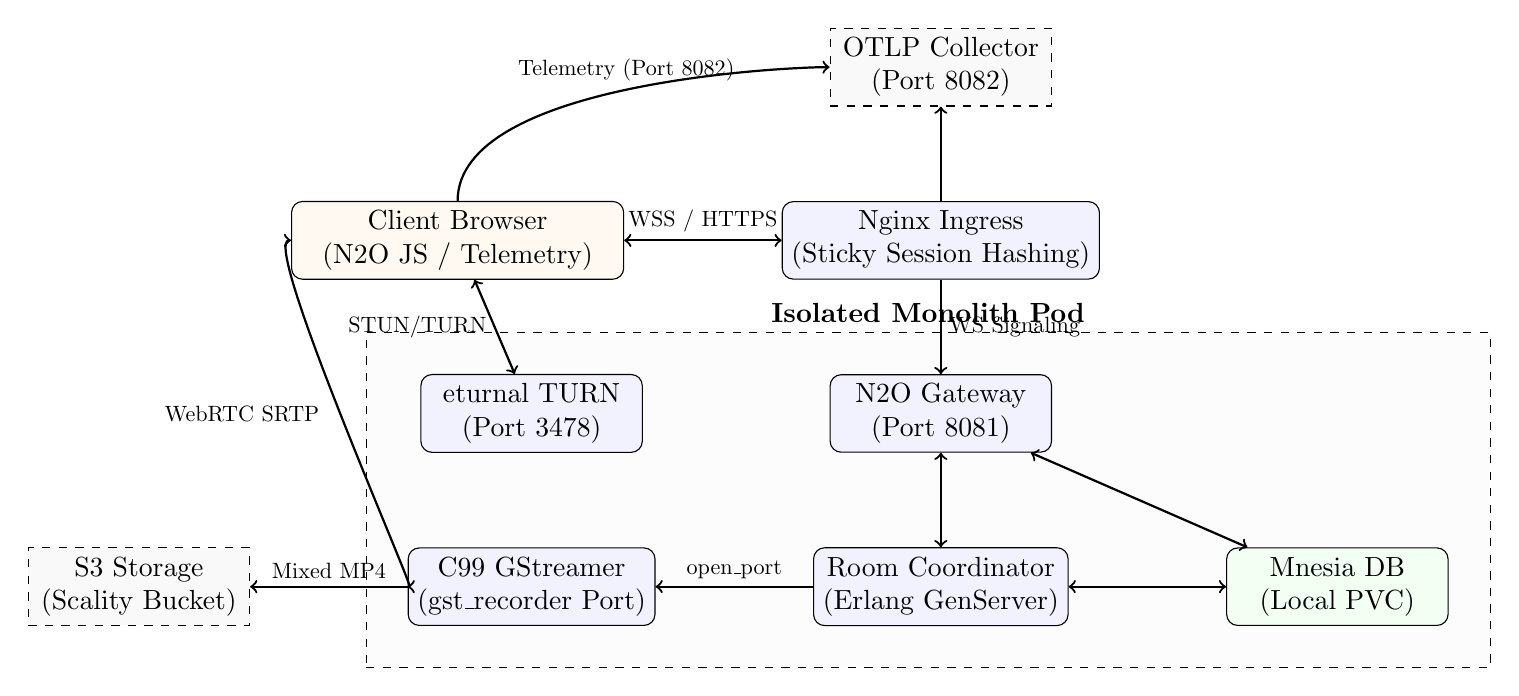
\begin{tikzpicture}[
    node distance=1.2cm and 1.5cm,
    block/.style={draw, rectangle, minimum height=2.8em, minimum width=8em, align=center, fill=blue!5, rounded corners},
    database/.style={draw, rectangle, minimum height=2.8em, minimum width=8em, fill=green!5, align=center, rounded corners},
    client/.style={draw, rounded corners, minimum height=2.8em, minimum width=12em, fill=orange!5, align=center},
    ext/.style={draw, dashed, rectangle, minimum height=2.8em, minimum width=8em, fill=gray!5, align=center}
]
    % Node definition (Constraint Based Relative Positioning - Swapped Mnesia and GStreamer)
    \node[client] (browser) {Client Browser \\ (N2O JS / Telemetry)};
    \node[block, right=of browser, xshift=0.5cm] (ingress) {Nginx Ingress \\ (Sticky Session Hashing)};
    \node[ext, above=of ingress] (otel) {OTLP Collector \\ (Port 8082)};
    % Isolated Monolith Pod boundary nodes
    \node[block, below=of ingress] (n2o) {N2O Gateway \\ (Port 8081)};
    \node[block, below=of n2o] (coord) {Room Coordinator \\ (Erlang GenServer)};
    % Swapped Positions: gst on left, mnesia on right
    \node[block, left=of coord, xshift=-0.5cm] (gst) {C99 GStreamer \\ (gst\_recorder Port)};
    \node[block, above=of gst] (eturnal) {eturnal TURN \\ (Port 3478)};
    \node[database, right=of coord, xshift=0.5cm] (mnesia) {Mnesia DB \\ (Local PVC)};
    % Grouping the Monolith Pod
    \begin{scope}[on background layer]
        \node[draw, dashed, fill=gray!2, inner sep=15pt, fit=(n2o) (coord) (mnesia) (eturnal) (gst), label=above:\textbf{Isolated Monolith Pod}] (pod) {};
    \end{scope}
    % Swapped S3 Storage position to far left to maintain planarity
    \node[ext, left=of gst, xshift=-0.5cm] (s3) {S3 Storage \\ (Scality Bucket)};
    % Arrows / Connections (Constraint Based Swapped Planar Connections)
    \draw[thick, <->] (browser) -- node[above, scale=0.8] {WSS / HTTPS} (ingress);
    \draw[thick, ->] (ingress) -- node[right, scale=0.8] {WS Signaling} (n2o);
    \draw[thick, ->] (ingress) -- (otel);
    % Planar Bezier curves and relative paths
    \draw[thick, <->] (browser) -- node[left, scale=0.8] {STUN/TURN} (eturnal);
    % Telemetry sweeping curve
    \draw[thick, ->] (browser) .. controls +(up:2.0cm) and +(left:2.0cm) .. node[above, scale=0.8] {Telemetry (Port 8082)} (otel);
    % Pod inner connections
    \draw[thick, <->] (n2o) -- (coord);
    \draw[thick, <->] (n2o) -- (mnesia);
    \draw[thick, <->] (coord) -- (mnesia);
    \draw[thick, ->] (coord) -- node[above, scale=0.8] {open\_port} (gst);
    \draw[thick, ->] (gst) -- node[above, scale=0.8] {Mixed MP4} (s3);
    % Planar curve for WebRTC SRTP media streams to left-placed gst node
    \draw[thick, <->] (browser) .. controls +(left:2.5cm) and +(left:1.5cm) .. node[left, scale=0.8, xshift=-0.2cm] {WebRTC SRTP} (gst);
\end{tikzpicture}
\caption{System topology planar graph layout with swapped database and media broker components. Avoids line crossings through relative constraints.}
\label{fig:topology}
\end{figure}

\subsection{Ingress Sticky Routing \& Room Sharding}
To scale the horizontal architecture to 1,000+ concurrent rooms, we bypass Erlang distribution. The Ingress proxy (Nginx or Envoy) parses the Room ID from the connection URI path (e.g., \texttt{/room/\{room\_id\}/signaling}) and maps it to a consistent target pod IP using a hash ring:
\begin{equation}
\text{Pod IP} = \text{Hash}(\text{room\_id}) \pmod P
\end{equation}
Where $P$ is the total count of running replicas. This ensures that:
\begin{itemize}
    \item All participants (judges, witnesses, jury members) of a specific room land on the same pod.
    \item The room signaling pub/sub is fully handled in-memory locally using N2O.
    \item The Erlang nodes run with \texttt{-no\_distribution}, avoiding the $O(P^2)$ cluster link storm.
    \item Mnesia acts as a purely local persistent transaction ledger mounted on an Alpine Linux local directory PVC.
\end{itemize}

\section{WebRTC Signaling Loop \& C99 Port Protocol}
The C99 GStreamer binary (\texttt{gst\_recorder}) is spawned as an OS process by the Erlang supervisor. Rather than linking against heavy socket libraries, it reads signaling data from \texttt{stdin} and outputs event payloads to \texttt{stdout}.

\subsection{Protocol Stack and Specifications}
The monolith interfaces utilize a diverse set of network and inter-process communication (IPC) protocols to coordinate signaling, manage media routing, and report client telemetry. Table~\ref{tab:protocols} provides a comprehensive description of each protocol, its transport layer, and operational parameters.

\begin{table}[h]
\centering
\caption{System Protocols and Inter-Process Specifications}
\label{tab:protocols}
\begin{tabular}{lp{3.2cm}p{4.0cm}p{4.8cm}}
\toprule
Protocol & Layer / Port & Primary Data Formats & Functional Description \\
\midrule
\textbf{GST Port (IPC)} & stdin/stdout Pipes & Line-delimited JSON & Custom Erlang-to-C99 binary signaling exchange for SDP offers/answers and ICE candidates. \\
\textbf{WS Signaling} & WSS / Port 8081 & Binary/Text over WebSocket & Cowboy/N2O room pub/sub channel for user joins, leaves, and chat logs. \\
\textbf{WebRTC SDP} & Signaling Channel & SDP Text (RFC 8866) & Session negotiation declaring codecs (H.264/VP8/Opus) and media directions. \\
\textbf{WebRTC ICE} & STUN/TURN (RFC 8489) & STUN Binding Attributes & Dynamic network connectivity probe establishing optimal media pathways. \\
\textbf{TURN Relay} & UDP/TCP / Port 3478 & STUN/TURN Relayed Packets & Relays encrypted SRTP media packets through \texttt{eturnal} when NAT/firewalls block P2P. \\
\textbf{SRTP / SRTCP} & UDP / Dynamic Ports & Encrypted RTP / RTCP (RFC 3711) & Transports secure real-time audio and video tracks between endpoints and GStreamer. \\
\textbf{QoS Telemetry} & HTTPS/WSS / Port 8082 & OTLP JSON / Protobuf & Prioritized client connection statistics pumped to OpenTelemetry collector. \\
\bottomrule
\end{tabular}
\end{table}

\subsection{Signaling Sequence Flow}
Figure~\ref{fig:sequence} illustrates the signaling loop during room startup, WebRTC negotiation, media composition, and session finalization.

\begin{figure}[h]
\centering
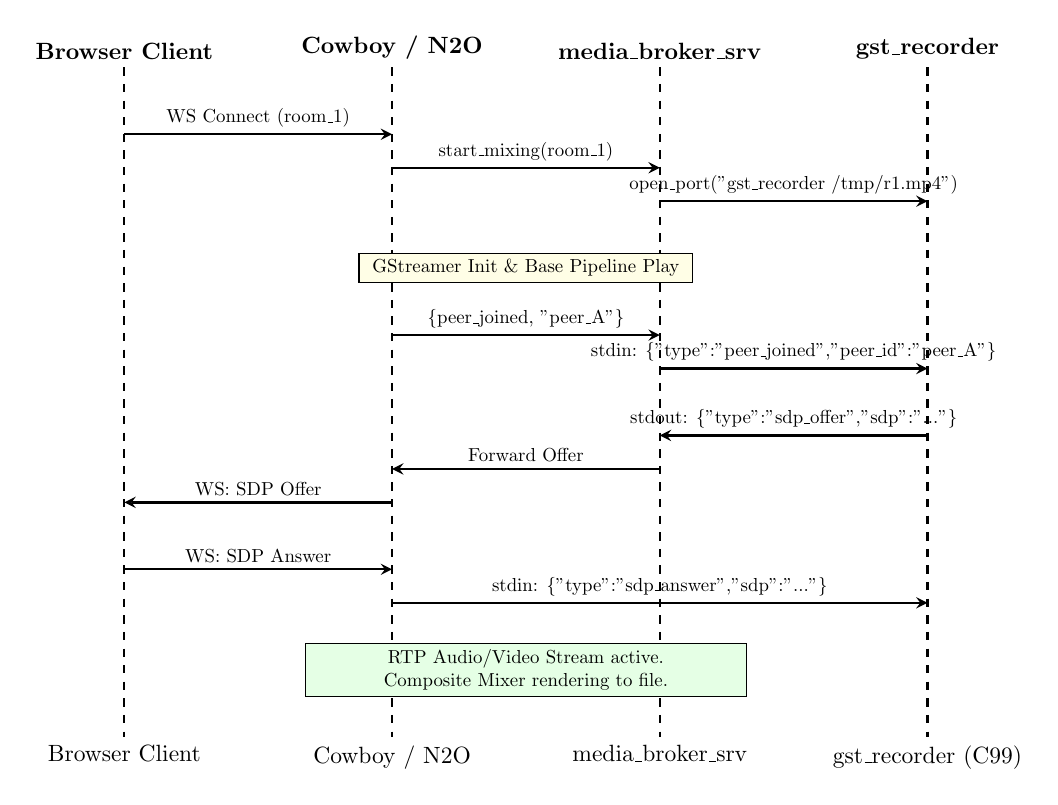
\begin{tikzpicture}[
    scale=0.85, every node/.style={transform shape},
    line/.style={draw, thick, dashed},
    arrow/.style={draw, thick, ->, >=stealth}
]
    % Lifelines
    \draw[line] (0,0) -- (0,-10) node[below] {Browser Client};
    \draw[line] (4,0) -- (4,-10) node[below] {Cowboy / N2O};
    \draw[line] (8,0) -- (8,-10) node[below] {media\_broker\_srv};
    \draw[line] (12,0) -- (12,-10) node[below] {gst\_recorder (C99)};

    % Headings
    \node[above] at (0,0) {\textbf{Browser Client}};
    \node[above] at (4,0) {\textbf{Cowboy / N2O}};
    \node[above] at (8,0) {\textbf{media\_broker\_srv}};
    \node[above] at (12,0) {\textbf{gst\_recorder}};

    % Step 1
    \draw[arrow] (0,-1) -- node[above, scale=0.8] {WS Connect (room\_1)} (4,-1);
    \draw[arrow] (4,-1.5) -- node[above, scale=0.8] {start\_mixing(room\_1)} (8,-1.5);
    \draw[arrow] (8,-2) -- node[above, scale=0.8] {open\_port("gst\_recorder /tmp/r1.mp4")} (12,-2);

    % Step 2
    \node[draw, fill=yellow!10, text width=6cm, align=center, scale=0.8] at (6,-3) {GStreamer Init \& Base Pipeline Play};
    
    % Step 3
    \draw[arrow] (4,-4) -- node[above, scale=0.8] {\{peer\_joined, "peer\_A"\}} (8,-4);
    \draw[arrow] (8,-4.5) -- node[above, scale=0.8] {stdin: \{"type":"peer\_joined","peer\_id":"peer\_A"\}} (12,-4.5);
    
    % Step 4
    \draw[arrow] (12,-5.5) -- node[above, scale=0.8] {stdout: \{"type":"sdp\_offer","sdp":"..."\}} (8,-5.5);
    \draw[arrow] (8,-6) -- node[above, scale=0.8] {Forward Offer} (4,-6);
    \draw[arrow] (4,-6.5) -- node[above, scale=0.8] {WS: SDP Offer} (0,-6.5);

    % Step 5
    \draw[arrow] (0,-7.5) -- node[above, scale=0.8] {WS: SDP Answer} (4,-7.5);
    \draw[arrow] (4,-8) -- node[above, scale=0.8] {stdin: \{"type":"sdp\_answer","sdp":"..."\}} (12,-8);

    % Step 6
    \node[draw, fill=green!10, text width=8cm, align=center, scale=0.8] at (6,-9) {RTP Audio/Video Stream active. Composite Mixer rendering to file.};

\end{tikzpicture}
\caption{Signaling sequence showing local Port I/O communication between Erlang and the C99 GStreamer binary.}
\label{fig:sequence}
\end{figure}

\section{Multipoint Media Composition Model}
The GStreamer media broker executes video grid compositing and audio conferencing concurrently.

\subsection{Video Matrix Grid Compositing}
Incoming H.264/VP8 video packets are decoded into raw YUV frames. The compositor element (\texttt{mix}) maps each input stream index $i \in \{0, 1, 2, 3\}$ to a quadrant layout inside a unified 1080p canvas ($W_{\text{out}} = 1920$, $H_{\text{out}} = 1080$). The dimensions of each video frame are scaled to $w = 960$ and $h = 540$. The placement coordinates $(x_i, y_i)$ are formulated as:
\begin{align}
x_i &= (i \pmod 2) \cdot w \\
y_i &= \lfloor i / 2 \rfloor \cdot h
\end{align}
The resulting video layout is composed as shown in Equation~\ref{eq:layout}:
\begin{equation}\label{eq:layout}
\text{Canvas}[x, y] = 
\begin{cases} 
\text{Stream}_0[x, y] & 0 \le x < 960,\ 0 \le y < 540 \\
\text{Stream}_1[x - 960, y] & 960 \le x < 1920,\ 0 \le y < 540 \\
\text{Stream}_2[x, y - 540] & 0 \le x < 960,\ 540 \le y < 1080 \\
\text{Stream}_3[x - 960, y - 540] & 960 \le x < 1920,\ 540 \le y < 1080
\end{cases}
\end{equation}

\subsection{Audio Mixing \& Summation}
Audio tracks are mixed using GStreamer's \texttt{audiomixer} element. Incoming Opus packets are decoded into linear pulse-code modulated (LPCM) audio buffers. The mixed audio signal $S_{\text{mixed}}(t)$ at timestamp $t$ is the sum of the $K$ active participant signals:
\begin{equation}
S_{\text{mixed}}(t) = \sum_{i=1}^{K} S_i(t)
\end{equation}
To prevent digital clipping/overflow, the mixed LPCM buffer passes through a limiter/clipper stage before being re-encoded into Opus for WebRTC downstream broadcast:
\begin{equation}
S_{\text{output}}(t) = \text{Clamp}(S_{\text{mixed}}(t), -S_{\text{max}}, S_{\text{max}})
\end{equation}

\section{Capacity \& SRE Metrics}
Table~\ref{tab:codecs_mcu} specifies the streaming codec, resolution, and bitrates assumed in our capacity review.

\begin{table}[h]
\centering
\caption{Codec, Resolution, and Bitrate Parameters}
\label{tab:codecs_mcu}
\begin{tabular}{llll}
\toprule
Stream Type & Codec & Resolution & Bitrate (per stream) \\
\midrule
Incoming WebRTC (per client) & H.264 (Baseline Profile) or VP8 & 720p ($1280 \times 720$) @ 30~fps & 1.5~Mbps \\
Output Recording (Composited) & H.264 (High Profile) via x264 & 1080p ($1920 \times 1080$) @ 30~fps & 4.0~Mbps \\
\bottomrule
\end{tabular}
\end{table}

Under a standard Kubernetes pod boundary of \textbf{4 CPU Cores} and \textbf{4 GB RAM}, software-based x264 compositing is compute-bound, limiting pod capacity to \textbf{3 active mixing rooms} (each room mixer requiring $\approx 1.0$ Core). To scale to 50 active rooms, the cluster leverages Ingress-based sharding across \textbf{17 stateless replicas}. Offloading the x264 encoder to hardware-accelerated NVENC interfaces on GPU-enabled nodes (reducing per-room complexity to $0.40$ Cores) allows a single 20-Core pod to host all 50 rooms.

\section{Conclusion}
The \texttt{rtp-monolith} architecture demonstrates that video conferencing signaling and media composting can be consolidated into a share-nothing Erlang/GStreamer node. By replacing microservice networks and headless browsers with local C99 OS port interfaces and Ingress Room Sticky Sessions, the system avoids cluster synchronization locks and mesh overhead. This provides a highly resilient, cost-effective SRE model for secure judicial networks.

\end{document}
